\chapter{Análisis amortizado}

\index{análisis amortizado}

La complejidad temporal de un algoritmo
a menudo es fácil de analizar
simplemente examinando la estructura
del algoritmo:
qué bucles contiene el algoritmo
y cuántas veces se realizan los bucles.
Sin embargo, a veces un análisis directo
no proporciona una imagen real de la eficiencia del algoritmo.

El \key{análisis amortizado} se puede utilizar para analizar
algoritmos que contienen operaciones cuya
complejidad temporal varía.
La idea es estimar el tiempo total utilizado en
todas estas operaciones durante la
ejecución del algoritmo, en lugar de centrarse
en operaciones individuales.

\section{Método de dos punteros}

\index{dos punteros}

En el \key{método de dos punteros},
se utilizan dos punteros para
iterar a través de los valores del arreglo.
Ambos punteros pueden moverse en una dirección solamente,
lo que garantiza que el algoritmo funcione de manera eficiente.
A continuación, discutimos dos problemas que se pueden resolver
utilizando el método de dos punteros.

\subsubsection{Suma en subarreglo}

Como primer ejemplo,
consideremos un problema en el que se nos da
un arreglo de $n$ enteros positivos
y una suma objetivo $x$,
y queremos encontrar un subarreglo cuya suma sea $x$
o informar que no existe tal subarreglo.

Por ejemplo, el arreglo
\begin{center}
    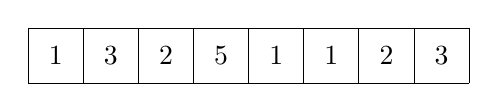
\begin{tikzpicture}[scale=0.7]
        \draw (0,0) grid (8,1);

        \node at (0.5,0.5) {$1$};
        \node at (1.5,0.5) {$3$};
        \node at (2.5,0.5) {$2$};
        \node at (3.5,0.5) {$5$};
        \node at (4.5,0.5) {$1$};
        \node at (5.5,0.5) {$1$};
        \node at (6.5,0.5) {$2$};
        \node at (7.5,0.5) {$3$};
    \end{tikzpicture}
\end{center}
contiene un subarreglo cuya suma es 8:
\begin{center}
    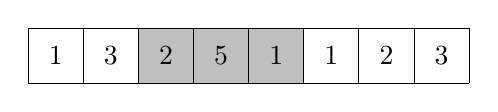
\begin{tikzpicture}[scale=0.7]
        \fill[color=lightgray] (2,0) rectangle (5,1);
        \draw (0,0) grid (8,1);

        \node at (0.5,0.5) {$1$};
        \node at (1.5,0.5) {$3$};
        \node at (2.5,0.5) {$2$};
        \node at (3.5,0.5) {$5$};
        \node at (4.5,0.5) {$1$};
        \node at (5.5,0.5) {$1$};
        \node at (6.5,0.5) {$2$};
        \node at (7.5,0.5) {$3$};
    \end{tikzpicture}
\end{center}

Este problema se puede resolver en tiempo
$O(n)$ utilizando el método de dos punteros.
La idea es mantener punteros que apuntan al
primer y último valor de un subarreglo.
En cada turno, el puntero izquierdo se mueve un paso
a la derecha, y el puntero derecho se mueve a la derecha
siempre que la suma del subarreglo resultante sea como máximo $x$.
Si la suma se convierte exactamente en $x$,
se ha encontrado una solución.

Por ejemplo, considera el siguiente arreglo
y una suma objetivo $x=8$:
\begin{center}
    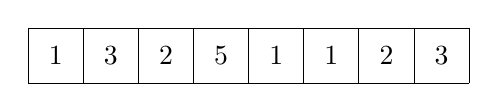
\begin{tikzpicture}[scale=0.7]
        \draw (0,0) grid (8,1);

        \node at (0.5,0.5) {$1$};
        \node at (1.5,0.5) {$3$};
        \node at (2.5,0.5) {$2$};
        \node at (3.5,0.5) {$5$};
        \node at (4.5,0.5) {$1$};
        \node at (5.5,0.5) {$1$};
        \node at (6.5,0.5) {$2$};
        \node at (7.5,0.5) {$3$};
    \end{tikzpicture}
\end{center}

El subarreglo inicial contiene los valores
1, 3 y 2 cuya suma es 6:

\begin{center}
    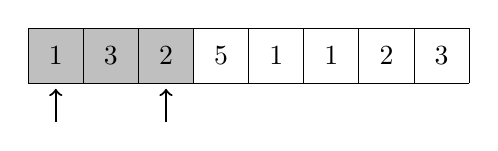
\begin{tikzpicture}[scale=0.7]
        \fill[color=lightgray] (0,0) rectangle (3,1);
        \draw (0,0) grid (8,1);

        \node at (0.5,0.5) {$1$};
        \node at (1.5,0.5) {$3$};
        \node at (2.5,0.5) {$2$};
        \node at (3.5,0.5) {$5$};
        \node at (4.5,0.5) {$1$};
        \node at (5.5,0.5) {$1$};
        \node at (6.5,0.5) {$2$};
        \node at (7.5,0.5) {$3$};

        \draw[thick,->] (0.5,-0.7) -- (0.5,-0.1);
        \draw[thick,->] (2.5,-0.7) -- (2.5,-0.1);
    \end{tikzpicture}
\end{center}

Luego, el puntero izquierdo se mueve un paso a la derecha.
El puntero derecho no se mueve, porque de lo contrario
la suma del subarreglo excedería $x$.

\begin{center}
    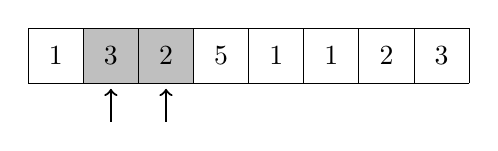
\begin{tikzpicture}[scale=0.7]
        \fill[color=lightgray] (1,0) rectangle (3,1);
        \draw (0,0) grid (8,1);

        \node at (0.5,0.5) {$1$};
        \node at (1.5,0.5) {$3$};
        \node at (2.5,0.5) {$2$};
        \node at (3.5,0.5) {$5$};
        \node at (4.5,0.5) {$1$};
        \node at (5.5,0.5) {$1$};
        \node at (6.5,0.5) {$2$};
        \node at (7.5,0.5) {$3$};

        \draw[thick,->] (1.5,-0.7) -- (1.5,-0.1);
        \draw[thick,->] (2.5,-0.7) -- (2.5,-0.1);
    \end{tikzpicture}
\end{center}

De nuevo, el puntero izquierdo se mueve un paso a la derecha,
y esta vez el puntero derecho se mueve tres
pasos a la derecha.
La suma del subarreglo es $2+5+1=8$, entonces se ha encontrado un subarreglo
cuya suma es $x$.

\begin{center}
    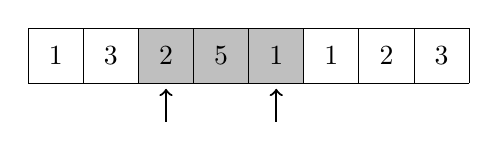
\begin{tikzpicture}[scale=0.7]
        \fill[color=lightgray] (2,0) rectangle (5,1);
        \draw (0,0) grid (8,1);

        \node at (0.5,0.5) {$1$};
        \node at (1.5,0.5) {$3$};
        \node at (2.5,0.5) {$2$};
        \node at (3.5,0.5) {$5$};
        \node at (4.5,0.5) {$1$};
        \node at (5.5,0.5) {$1$};
        \node at (6.5,0.5) {$2$};
        \node at (7.5,0.5) {$3$};

        \draw[thick,->] (2.5,-0.7) -- (2.5,-0.1);
        \draw[thick,->] (4.5,-0.7) -- (4.5,-0.1);
    \end{tikzpicture}
\end{center}

El tiempo de ejecución del algoritmo depende de
la cantidad de pasos que el puntero derecho se mueva.
Si bien no hay un límite superior útil sobre cuántos pasos puede
moverse el puntero en un \emph{único} turno,
sabemos que el puntero se mueve \emph{un total de}
$O(n)$ pasos durante el algoritmo,
porque solo se mueve hacia la derecha.

Dado que tanto el puntero izquierdo como el derecho
se mueven $O(n)$ pasos durante el algoritmo,
el algoritmo funciona en tiempo $O(n)$.

\subsubsection{Problema 2SUM}

Otro problema que se puede resolver usando
el método de dos punteros es el siguiente problema,
también conocido como el problema \key{2SUM}:
dado un arreglo de $n$ números y
una suma objetivo $x$, encuentre
dos valores del arreglo tales que su suma sea $x$,
o informe que no existen tales valores.

Para resolver el problema, primero
ordenamos los valores del arreglo en orden creciente.
Después de eso, iteramos a través del arreglo usando
dos punteros.
El puntero izquierdo comienza en el primer valor
y se mueve un paso a la derecha en cada turno.
El puntero derecho comienza en el último valor
y siempre se mueve hacia la izquierda hasta que la suma de los
valores izquierdo y derecho sea como máximo $x$.
Si la suma es exactamente $x$,
se ha encontrado una solución.

\pagebreak
Por ejemplo, considera el siguiente arreglo
y una suma objetivo $x=12$:
\begin{center}
    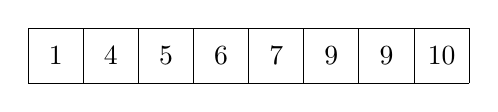
\begin{tikzpicture}[scale=0.7]
        \draw (0,0) grid (8,1);

        \node at (0.5,0.5) {$1$};
        \node at (1.5,0.5) {$4$};
        \node at (2.5,0.5) {$5$};
        \node at (3.5,0.5) {$6$};
        \node at (4.5,0.5) {$7$};
        \node at (5.5,0.5) {$9$};
        \node at (6.5,0.5) {$9$};
        \node at (7.5,0.5) {$10$};
    \end{tikzpicture}
\end{center}

Las posiciones iniciales de los punteros
son las siguientes.
La suma de los valores es $1+10=11$
que es menor que $x$.

\begin{center}
    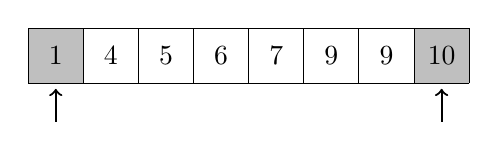
\begin{tikzpicture}[scale=0.7]
        \fill[color=lightgray] (0,0) rectangle (1,1);
        \fill[color=lightgray] (7,0) rectangle (8,1);
        \draw (0,0) grid (8,1);

        \node at (0.5,0.5) {$1$};
        \node at (1.5,0.5) {$4$};
        \node at (2.5,0.5) {$5$};
        \node at (3.5,0.5) {$6$};
        \node at (4.5,0.5) {$7$};
        \node at (5.5,0.5) {$9$};
        \node at (6.5,0.5) {$9$};
        \node at (7.5,0.5) {$10$};

        \draw[thick,->] (0.5,-0.7) -- (0.5,-0.1);
        \draw[thick,->] (7.5,-0.7) -- (7.5,-0.1);
    \end{tikzpicture}
\end{center}

Luego, el puntero izquierdo se mueve un paso a la derecha.
El puntero derecho se mueve tres pasos a la izquierda,
y la suma se convierte en $4+7=11$.

\begin{center}
    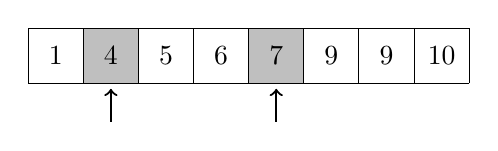
\begin{tikzpicture}[scale=0.7]
        \fill[color=lightgray] (1,0) rectangle (2,1);
        \fill[color=lightgray] (4,0) rectangle (5,1);
        \draw (0,0) grid (8,1);

        \node at (0.5,0.5) {$1$};
        \node at (1.5,0.5) {$4$};
        \node at (2.5,0.5) {$5$};
        \node at (3.5,0.5) {$6$};
        \node at (4.5,0.5) {$7$};
        \node at (5.5,0.5) {$9$};
        \node at (6.5,0.5) {$9$};
        \node at (7.5,0.5) {$10$};

        \draw[thick,->] (1.5,-0.7) -- (1.5,-0.1);
        \draw[thick,->] (4.5,-0.7) -- (4.5,-0.1);
    \end{tikzpicture}
\end{center}

Después de esto, el puntero izquierdo se mueve un paso a la derecha nuevamente.
El puntero derecho no se mueve y se encuentra una solución
$5+7=12$.

\begin{center}
    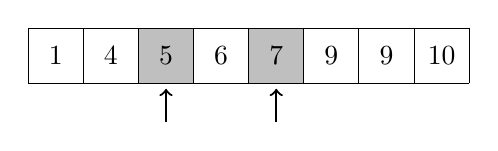
\begin{tikzpicture}[scale=0.7]
        \fill[color=lightgray] (2,0) rectangle (3,1);
        \fill[color=lightgray] (4,0) rectangle (5,1);
        \draw (0,0) grid (8,1);

        \node at (0.5,0.5) {$1$};
        \node at (1.5,0.5) {$4$};
        \node at (2.5,0.5) {$5$};
        \node at (3.5,0.5) {$6$};
        \node at (4.5,0.5) {$7$};
        \node at (5.5,0.5) {$9$};
        \node at (6.5,0.5) {$9$};
        \node at (7.5,0.5) {$10$};

        \draw[thick,->] (2.5,-0.7) -- (2.5,-0.1);
        \draw[thick,->] (4.5,-0.7) -- (4.5,-0.1);
    \end{tikzpicture}
\end{center}

El tiempo de ejecución del algoritmo es
$O(n \log n)$, porque primero ordena
el arreglo en tiempo $O(n \log n)$,
y luego ambos punteros se mueven $O(n)$ pasos.

Ten en cuenta que es posible resolver el problema
de otra manera en tiempo $O(n \log n)$ usando búsqueda binaria.
En tal solución, iteramos a través del arreglo
y para cada valor del arreglo, intentamos encontrar otro
valor que produzca la suma $x$.
Esto se puede hacer realizando $n$ búsquedas binarias,
cada una de las cuales toma tiempo $O(\log n)$.

Un problema más difícil es
el \key{problema 3SUM}, que pide
encontrar \emph{tres} valores del arreglo
cuya suma sea $x$.
Usando la idea del algoritmo anterior,
este problema se puede resolver en tiempo $O(n^2)$.\footnote{Durante mucho tiempo,
    se pensó que resolver
    el problema 3SUM de manera más eficiente que en tiempo $O(n^2)$
    no sería posible.
    Sin embargo, en 2014, resultó \cite{gro14}
    que este no es el caso.}
¿Puedes ver cómo?

\section{Elementos menores más cercanos}

\index{elementos menores más cercanos}

El análisis amortizado se utiliza a menudo para
estimar el número de operaciones
realizadas en una estructura de datos.
Las operaciones pueden distribuirse de manera desigual de modo que
la mayoría de las operaciones ocurran durante una
fase específica del algoritmo, pero el número total
de operaciones está limitado.

Como ejemplo, considera el problema
de encontrar para cada elemento del arreglo
el \key{elemento menor más cercano}, es decir,
el primer elemento menor que precede al elemento
en el arreglo.
Es posible que no exista tal elemento,
en cuyo caso el algoritmo debe informarlo.
A continuación veremos cómo el problema puede ser
resuelto eficientemente utilizando una estructura de pila.

Recorremos el arreglo de izquierda a derecha
y mantenemos una pila de elementos del arreglo.
En cada posición del arreglo, eliminamos elementos de la pila
hasta que el elemento superior sea menor que el
elemento actual, o la pila esté vacía.
Luego, informamos que el elemento superior es
el elemento menor más cercano del elemento actual,
o si la pila está vacía, no existe tal elemento.
Finalmente, agregamos el elemento actual a la pila.

Como ejemplo, considera el siguiente arreglo:
\begin{center}
    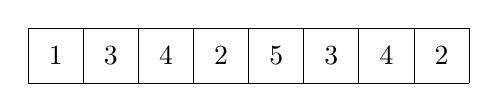
\begin{tikzpicture}[scale=0.7]
        \draw (0,0) grid (8,1);

        \node at (0.5,0.5) {$1$};
        \node at (1.5,0.5) {$3$};
        \node at (2.5,0.5) {$4$};
        \node at (3.5,0.5) {$2$};
        \node at (4.5,0.5) {$5$};
        \node at (5.5,0.5) {$3$};
        \node at (6.5,0.5) {$4$};
        \node at (7.5,0.5) {$2$};
    \end{tikzpicture}
\end{center}

Primero, los elementos 1, 3 y 4 se agregan a la pila,
porque cada elemento es mayor que el elemento anterior.
Por lo tanto, el elemento menor más cercano de 4 es 3,
y el elemento menor más cercano de 3 es 1.
\begin{center}
    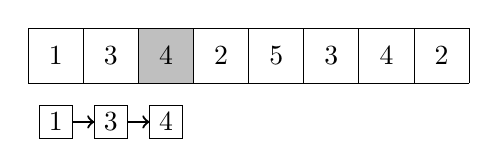
\begin{tikzpicture}[scale=0.7]
        \fill[color=lightgray] (2,0) rectangle (3,1);
        \draw (0,0) grid (8,1);

        \node at (0.5,0.5) {$1$};
        \node at (1.5,0.5) {$3$};
        \node at (2.5,0.5) {$4$};
        \node at (3.5,0.5) {$2$};
        \node at (4.5,0.5) {$5$};
        \node at (5.5,0.5) {$3$};
        \node at (6.5,0.5) {$4$};
        \node at (7.5,0.5) {$2$};

        \draw (0.2,0.2-1.2) rectangle (0.8,0.8-1.2);
        \draw (1.2,0.2-1.2) rectangle (1.8,0.8-1.2);
        \draw (2.2,0.2-1.2) rectangle (2.8,0.8-1.2);

        \node at (0.5,0.5-1.2) {$1$};
        \node at (1.5,0.5-1.2) {$3$};
        \node at (2.5,0.5-1.2) {$4$};

        \draw[->,thick] (0.8,0.5-1.2) -- (1.2,0.5-1.2);
        \draw[->,thick] (1.8,0.5-1.2) -- (2.2,0.5-1.2);
    \end{tikzpicture}
\end{center}

El siguiente elemento 2 es menor que los dos elementos superiores
en la pila.
Por lo tanto, los elementos 3 y 4 se eliminan de la pila,
y luego el elemento 2 se agrega a la pila.
Su elemento menor más cercano es 1:
\begin{center}
    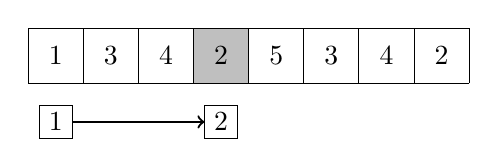
\begin{tikzpicture}[scale=0.7]
        \fill[color=lightgray] (3,0) rectangle (4,1);
        \draw (0,0) grid (8,1);

        \node at (0.5,0.5) {$1$};
        \node at (1.5,0.5) {$3$};
        \node at (2.5,0.5) {$4$};
        \node at (3.5,0.5) {$2$};
        \node at (4.5,0.5) {$5$};
        \node at (5.5,0.5) {$3$};
        \node at (6.5,0.5) {$4$};
        \node at (7.5,0.5) {$2$};

        \draw (0.2,0.2-1.2) rectangle (0.8,0.8-1.2);
        \draw (3.2,0.2-1.2) rectangle (3.8,0.8-1.2);

        \node at (0.5,0.5-1.2) {$1$};
        \node at (3.5,0.5-1.2) {$2$};

        \draw[->,thick] (0.8,0.5-1.2) -- (3.2,0.5-1.2);
    \end{tikzpicture}
\end{center}

Luego, el elemento 5 es mayor que el elemento 2,
así que se agregará a la pila, y
su elemento menor más cercano es 2:
\begin{center}
    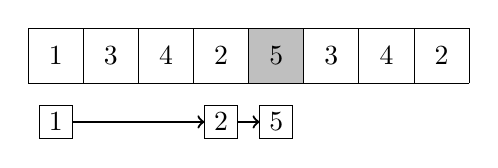
\begin{tikzpicture}[scale=0.7]
        \fill[color=lightgray] (4,0) rectangle (5,1);
        \draw (0,0) grid (8,1);

        \node at (0.5,0.5) {$1$};
        \node at (1.5,0.5) {$3$};
        \node at (2.5,0.5) {$4$};
        \node at (3.5,0.5) {$2$};
        \node at (4.5,0.5) {$5$};
        \node at (5.5,0.5) {$3$};
        \node at (6.5,0.5) {$4$};
        \node at (7.5,0.5) {$2$};

        \draw (0.2,0.2-1.2) rectangle (0.8,0.8-1.2);
        \draw (3.2,0.2-1.2) rectangle (3.8,0.8-1.2);
        \draw (4.2,0.2-1.2) rectangle (4.8,0.8-1.2);

        \node at (0.5,0.5-1.2) {$1$};
        \node at (3.5,0.5-1.2) {$2$};
        \node at (4.5,0.5-1.2) {$5$};

        \draw[->,thick] (0.8,0.5-1.2) -- (3.2,0.5-1.2);
        \draw[->,thick] (3.8,0.5-1.2) -- (4.2,0.5-1.2);
    \end{tikzpicture}
\end{center}

Después de esto, el elemento 5 se elimina de la pila
y los elementos 3 y 4 se agregan a la pila:
\begin{center}
    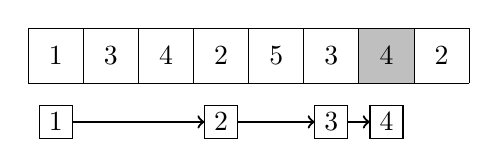
\begin{tikzpicture}[scale=0.7]
        \fill[color=lightgray] (6,0) rectangle (7,1);
        \draw (0,0) grid (8,1);

        \node at (0.5,0.5) {$1$};
        \node at (1.5,0.5) {$3$};
        \node at (2.5,0.5) {$4$};
        \node at (3.5,0.5) {$2$};
        \node at (4.5,0.5) {$5$};
        \node at (5.5,0.5) {$3$};
        \node at (6.5,0.5) {$4$};
        \node at (7.5,0.5) {$2$};

        \draw (0.2,0.2-1.2) rectangle (0.8,0.8-1.2);
        \draw (3.2,0.2-1.2) rectangle (3.8,0.8-1.2);
        \draw (5.2,0.2-1.2) rectangle (5.8,0.8-1.2);
        \draw (6.2,0.2-1.2) rectangle (6.8,0.8-1.2);

        \node at (0.5,0.5-1.2) {$1$};
        \node at (3.5,0.5-1.2) {$2$};
        \node at (5.5,0.5-1.2) {$3$};
        \node at (6.5,0.5-1.2) {$4$};

        \draw[->,thick] (0.8,0.5-1.2) -- (3.2,0.5-1.2);
        \draw[->,thick] (3.8,0.5-1.2) -- (5.2,0.5-1.2);
        \draw[->,thick] (5.8,0.5-1.2) -- (6.2,0.5-1.2);
    \end{tikzpicture}
\end{center}

Finalmente, todos los elementos excepto 1 son eliminados
de la pila y el último elemento 2
se agrega a la pila:

\begin{center}
    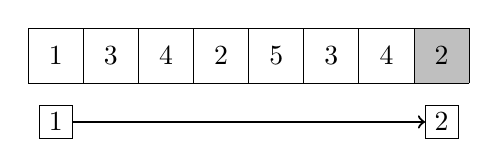
\begin{tikzpicture}[scale=0.7]
        \fill[color=lightgray] (7,0) rectangle (8,1);
        \draw (0,0) grid (8,1);

        \node at (0.5,0.5) {$1$};
        \node at (1.5,0.5) {$3$};
        \node at (2.5,0.5) {$4$};
        \node at (3.5,0.5) {$2$};
        \node at (4.5,0.5) {$5$};
        \node at (5.5,0.5) {$3$};
        \node at (6.5,0.5) {$4$};
        \node at (7.5,0.5) {$2$};

        \draw (0.2,0.2-1.2) rectangle (0.8,0.8-1.2);
        \draw (7.2,0.2-1.2) rectangle (7.8,0.8-1.2);

        \node at (0.5,0.5-1.2) {$1$};
        \node at (7.5,0.5-1.2) {$2$};

        \draw[->,thick] (0.8,0.5-1.2) -- (7.2,0.5-1.2);
    \end{tikzpicture}
\end{center}

La eficiencia del algoritmo depende del
número total de operaciones en la pila.
Si el elemento actual es más grande que
el elemento superior en la pila, se agrega directamente
a la pila, lo cual es eficiente.
Sin embargo, a veces la pila puede contener varios
elementos más grandes y lleva tiempo eliminarlos.
Aun así, cada elemento se agrega \emph{exactamente una vez} a la pila
y se elimina \emph{como máximo una vez} de la pila.
Por lo tanto, cada elemento causa $O(1)$ operaciones en la pila,
y el algoritmo funciona en tiempo $O(n)$.

\section{Mínimo en ventana deslizante}

\index{ventana deslizante}
\index{mínimo en ventana deslizante}

Una \key{ventana deslizante} es un subarreglo de tamaño constante
que se mueve de izquierda a derecha a través de un arreglo.
En cada posición de la ventana,
queremos calcular cierta información
sobre los elementos dentro de ella.
En esta sección, nos enfocamos en el problema
de mantener el \key{mínimo en ventana deslizante},
lo que significa que debemos informar el valor más
pequeño dentro de cada ventana.

El mínimo en ventana deslizante se puede calcular
usando una idea similar a la que utilizamos para calcular
los elementos menores más cercanos.
Mantenemos una cola
donde cada elemento es más grande que
el elemento anterior,
y el primer elemento
siempre corresponde al elemento mínimo dentro de la ventana.
Después de cada movimiento de ventana,
eliminamos elementos del final de la cola
hasta que el último elemento de la cola
sea más pequeño que el nuevo elemento de la ventana,
o la cola quede vacía.
También eliminamos el primer elemento de la cola
si ya no está dentro de la ventana.
Finalmente, agregamos el nuevo elemento de la ventana
al final de la cola.

Como ejemplo, considera el siguiente arreglo:

\begin{center}
    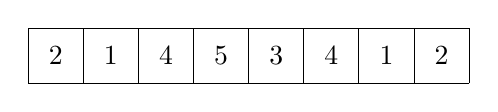
\begin{tikzpicture}[scale=0.7]
        \draw (0,0) grid (8,1);

        \node at (0.5,0.5) {$2$};
        \node at (1.5,0.5) {$1$};
        \node at (2.5,0.5) {$4$};
        \node at (3.5,0.5) {$5$};
        \node at (4.5,0.5) {$3$};
        \node at (5.5,0.5) {$4$};
        \node at (6.5,0.5) {$1$};
        \node at (7.5,0.5) {$2$};
    \end{tikzpicture}
\end{center}

Supongamos que el tamaño de la ventana deslizante es 4.
En la primera posición de la ventana, el valor más pequeño es 1:
\begin{center}
    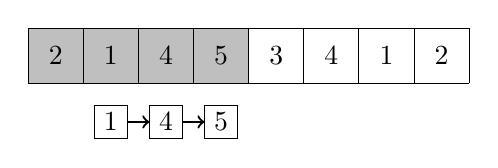
\begin{tikzpicture}[scale=0.7]
        \fill[color=lightgray] (0,0) rectangle (4,1);
        \draw (0,0) grid (8,1);

        \node at (0.5,0.5) {$2$};
        \node at (1.5,0.5) {$1$};
        \node at (2.5,0.5) {$4$};
        \node at (3.5,0.5) {$5$};
        \node at (4.5,0.5) {$3$};
        \node at (5.5,0.5) {$4$};
        \node at (6.5,0.5) {$1$};
        \node at (7.5,0.5) {$2$};

        \draw (1.2,0.2-1.2) rectangle (1.8,0.8-1.2);
        \draw (2.2,0.2-1.2) rectangle (2.8,0.8-1.2);
        \draw (3.2,0.2-1.2) rectangle (3.8,0.8-1.2);

        \node at (1.5,0.5-1.2) {$1$};
        \node at (2.5,0.5-1.2) {$4$};
        \node at (3.5,0.5-1.2) {$5$};

        \draw[->,thick] (1.8,0.5-1.2) -- (2.2,0.5-1.2);
        \draw[->,thick] (2.8,0.5-1.2) -- (3.2,0.5-1.2);
    \end{tikzpicture}
\end{center}

Luego, la ventana se mueve un paso a la derecha.
El nuevo elemento 3 es más pequeño que los elementos
4 y 5 en la cola, por lo que los elementos 4 y 5
se eliminan de la cola
y el elemento 3 se agrega a la cola.
El valor más pequeño sigue siendo 1.
\begin{center}
    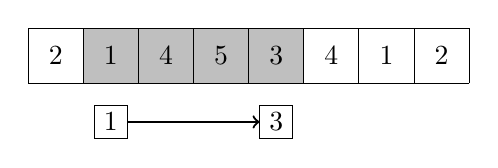
\begin{tikzpicture}[scale=0.7]
        \fill[color=lightgray] (1,0) rectangle (5,1);
        \draw (0,0) grid (8,1);

        \node at (0.5,0.5) {$2$};
        \node at (1.5,0.5) {$1$};
        \node at (2.5,0.5) {$4$};
        \node at (3.5,0.5) {$5$};
        \node at (4.5,0.5) {$3$};
        \node at (5.5,0.5) {$4$};
        \node at (6.5,0.5) {$1$};
        \node at (7.5,0.5) {$2$};

        \draw (1.2,0.2-1.2) rectangle (1.8,0.8-1.2);
        \draw (4.2,0.2-1.2) rectangle (4.8,0.8-1.2);

        \node at (1.5,0.5-1.2) {$1$};
        \node at (4.5,0.5-1.2) {$3$};

        \draw[->,thick] (1.8,0.5-1.2) -- (4.2,0.5-1.2);
    \end{tikzpicture}
\end{center}

\newpage
Después de esto, la ventana se mueve nuevamente,
y el elemento más pequeño 1
ya no pertenece a la ventana.
Por lo tanto, se elimina de la cola y ahora, el valor más pequeño
es 3. También se agrega el nuevo elemento 4
a la cola.
\begin{center}
    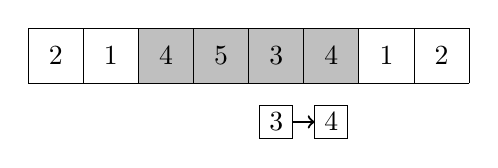
\begin{tikzpicture}[scale=0.7]
        \fill[color=lightgray] (2,0) rectangle (6,1);
        \draw (0,0) grid (8,1);

        \node at (0.5,0.5) {$2$};
        \node at (1.5,0.5) {$1$};
        \node at (2.5,0.5) {$4$};
        \node at (3.5,0.5) {$5$};
        \node at (4.5,0.5) {$3$};
        \node at (5.5,0.5) {$4$};
        \node at (6.5,0.5) {$1$};
        \node at (7.5,0.5) {$2$};

        \draw (4.2,0.2-1.2) rectangle (4.8,0.8-1.2);
        \draw (5.2,0.2-1.2) rectangle (5.8,0.8-1.2);

        \node at (4.5,0.5-1.2) {$3$};
        \node at (5.5,0.5-1.2) {$4$};

        \draw[->,thick] (4.8,0.5-1.2) -- (5.2,0.5-1.2);
    \end{tikzpicture}
\end{center}

El siguiente nuevo elemento 1 es más pequeño que todos los elementos
en la cola.
Por lo tanto, se eliminan todos los elementos de la cola
y solo contendrá el elemento 1:
\begin{center}
    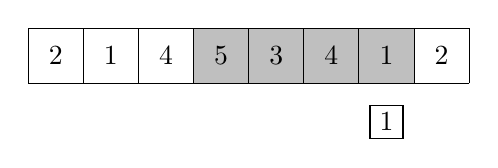
\begin{tikzpicture}[scale=0.7]
        \fill[color=lightgray] (3,0) rectangle (7,1);
        \draw (0,0) grid (8,1);

        \node at (0.5,0.5) {$2$};
        \node at (1.5,0.5) {$1$};
        \node at (2.5,0.5) {$4$};
        \node at (3.5,0.5) {$5$};
        \node at (4.5,0.5) {$3$};
        \node at (5.5,0.5) {$4$};
        \node at (6.5,0.5) {$1$};
        \node at (7.5,0.5) {$2$};

        \draw (6.2,0.2-1.2) rectangle (6.8,0.8-1.2);

        \node at (6.5,0.5-1.2) {$1$};
    \end{tikzpicture}
\end{center}

Finalmente, la ventana llega a su última posición.
El elemento 2 se agrega a la cola,
pero el valor más pequeño dentro de la ventana
sigue siendo 1.
\begin{center}
    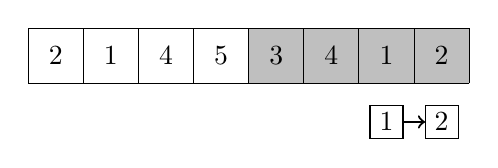
\begin{tikzpicture}[scale=0.7]
        \fill[color=lightgray] (4,0) rectangle (8,1);
        \draw (0,0) grid (8,1);

        \node at (0.5,0.5) {$2$};
        \node at (1.5,0.5) {$1$};
        \node at (2.5,0.5) {$4$};
        \node at (3.5,0.5) {$5$};
        \node at (4.5,0.5) {$3$};
        \node at (5.5,0.5) {$4$};
        \node at (6.5,0.5) {$1$};
        \node at (7.5,0.5) {$2$};

        \draw (6.2,0.2-1.2) rectangle (6.8,0.8-1.2);
        \draw (7.2,0.2-1.2) rectangle (7.8,0.8-1.2);

        \node at (6.5,0.5-1.2) {$1$};
        \node at (7.5,0.5-1.2) {$2$};

        \draw[->,thick] (6.8,0.5-1.2) -- (7.2,0.5-1.2);
    \end{tikzpicture}
\end{center}

Dado que cada elemento del arreglo
se agrega a la cola exactamente una vez y
se elimina de la cola como máximo una vez,
el algoritmo funciona en tiempo $O(n)$.


